\chapter{A ferramenta desenvolvida}

Para o desenvolvimento do software livraria Dom Casmurro foi utilizado as seguintes ferramentas:


\section{Linguagem de programação}
 A linguagem de programação utilizada foi a linguem Java, muito utilizada em desenvolvimento para desktop e web. É uma linguagem orientada a objetos,fortemente tipada e multiplataforma, de modo que uma vez compilado o código, é possivel executa-lo em qualquer sistema que disponha de uma maquina virtual Java;

\section{Ambiente de desenvolvimento}
 O ambiente utilizado para o desenvolvimento do código do programa foi o software NetBeans IDE versão 8.0.1; focada no desenvolvimento utilizando a linguagem de programação Java.

\section{Persistência de dados}
 O armazenamento das informações como por exemplo os cadastro das operações de cliente, funcionários, fornecedores e livros são inseridos no banco de dados Mysql Server 5.6;

O software utilizado para o desenvolvimento do banco de dados foi o MySQL Workbench 6.0 CE. Tem como função a modelagem e gerenciamento dos dados, onde gera as tabelas e seus relacionamentos, podendo inserir dados nessas tabelas e efetuar a sincronização entre modelo lógico e a base de dados física.


\section{Requisitos Funcionais}

\begin{itemize}

\item Ao abrir o software a tela de login é exibida, mostrando os campos “usuário” e “senha”, com dois botões, um “acessar” o software, e outro para “cancelar” a operação;

\item Se o botão “Cancelar” for pressionado é exibida uma mensagem de aviso: “Tem certeza que deseja encerrar a operação?” se “sim” a mensagem de aviso some e o programa é automaticamente fechado; se “não” a mensagem é fechada e permanece na tela de login;

\item Se o botão “Acessar” for pressionado o software verifica se a senha está correta: “empresa123”, a tela principal do software é exibida. E a tela de login é fechada. Caso a “senha” esteja incorreta o software exibe uma mensagem de aviso: “Senha incorreta” e limpa os campo para que possa ser novamente preenchido.

\item Na tela principal do software é exibido um menu com as seguintes informações “Cadastrar”, “Consultar”, “Editar”, “Deletar” e “sobre”;

\item Se qualquer uma das opções do menu for pressionado: será exibido um submenu: “Cliente”, “Funcionário”, “Fornecedor”, “Livros”;

\item No “cadastro” o usuário poderá cadastrar os “Cliente”, “Funcionário”, “Fornecedor”, “Livros”, na base de dados;

\item Na “Consulta” o usuário poderá ter acesso as informações armazenada na base de dados, de qualquer uma das opções mencionadas acima;

\item Em “Editar” o usuário poderá acrescentar, remover ou alterar informações dos cadastros feitos;

\item Caso seja necessário o menu com a opção “Deletar” fará com que o usuário possa remover os  cadastros realizados até o então.

\item Se  “Sobre” do menu principal for selecionado será exibido uma tela com as informações do software e quem o desenvolveu;


\end{itemize}


\section{Requisitos Não Funcionais}

\begin{itemize}

\item O software é deve ser desenvolvido na linguagem de programação Java, aproveitando sua natureza mutiplataforma e pela mesma fazer parte da ementa do curso Técnico em Informática;

\item Para executar nosso programa com sobra de recursos é necessário uma máquina com um processador Intel Atom de 1,7 GHZ com 2GB de memória RAM;

\item É executado em qualquer plataforma seja ela Linux, Windows;
\end{itemize}

\section {UML do software (Diagrama de USE CASE)}

A construção da UML no desenvolvimento do software trouxe vários benefícios, pois nos auxiliou na modelagem e 
documentação do sistema. Nele foi construído as definições de cada uma das operações. A figura \ref{uml_cliente}
representa o Diagrama de Casos de Uso do Cliente. A seguir tem-se a descrição de cada uma das açoes possíveis para
o cliente.

%=================================================================================

\begin{figure}[ht]
	\centering 
	\caption{UML Cliente}
	
	\label{uml_cliente}
	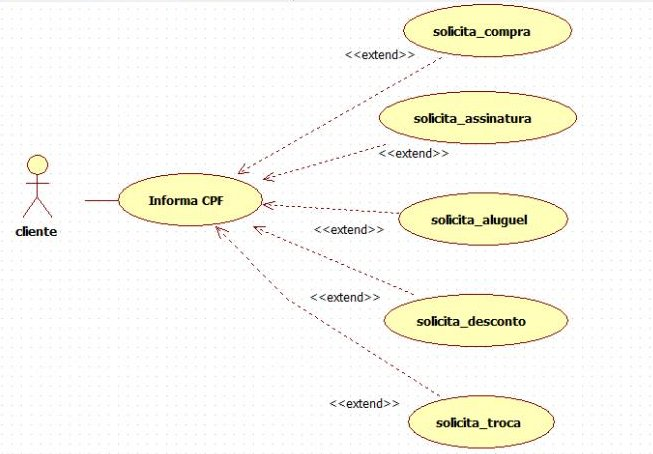
\includegraphics[scale = 0.7]{imagens/uml-cliente.jpg}
	\\Fonte: Do autor
\end{figure}


\begin{itemize}
\item Cliente informa seu CPF para o funcionários
\item Cliente solicitar uma compra de livros;
\item Cliente solicita assinatura mensal de livros;
\item Cliente solicita o aluguel dos livros;
\item Cliente solicita desconto na compra de um livro;
\item Cliente solicita a troca dos livros;
\end{itemize}

A figura \ref{uml_funcionario} representa o Diagrama de Casos de Uso do
Funcionário. A seguir tem-se a descrição de cada uma das açoes possíveis para
o usuário.

%=================================================================================
%UML FUNCIONARIO 

\begin{figure}[ht]
	\centering 
	\caption{UML Funcionario}
	\label{uml_funcionario}
	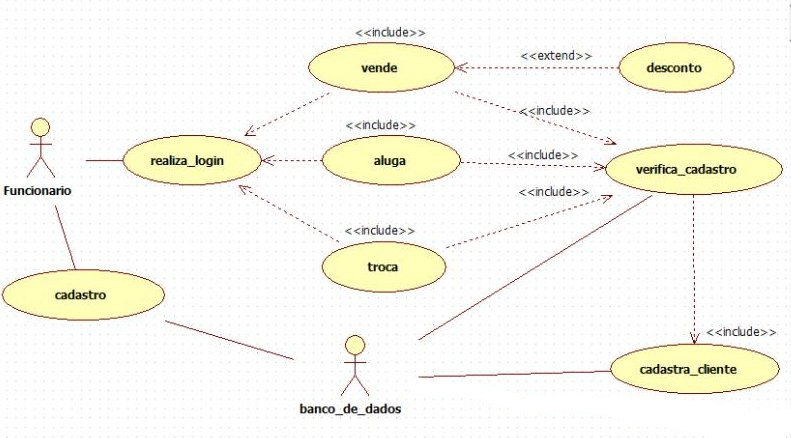
\includegraphics[scale = 0.50]{imagens/uml-funcionario.jpg}
	\\Fonte: Do autor
\end{figure}

\begin{itemize}
\item Funcionário realiza cadastro e armazena no banco de dados;
\item Funcionário realiza login no sistema;
\item Funcionário vende, troca, aluga livros para o cliente;
\item Funcionário oferece desconto na venda do livro;
\item Funcionário verifica o cadastro na venda, troca e aluguel dos livros;
\item Se cliente não for cadastrado: Funcionário cadastra Cliente no Banco de dados;
\end{itemize}

%=================================================================================
A figura \ref{uml_fornecedor} representa o Diagrama de Casos de Uso do
Fornecedor. A seguir tem-se a descrição de cada uma das açoes possíveis para
o fornecedor.

\begin{itemize}
\item Fornecedor informa CPF para o funcionário;
\item Se Fornecedor não cadastrado funcionário o cadastra no banco de dados;
\item Fornecedor vende livro para a empresa;
\item Fornecedor solicita desconto na venda dos livros;os;
\end{itemize}

\begin{figure}[h]
	\centering 
	\caption{UML Fornecedor}
	\label{uml_fornecedor}
	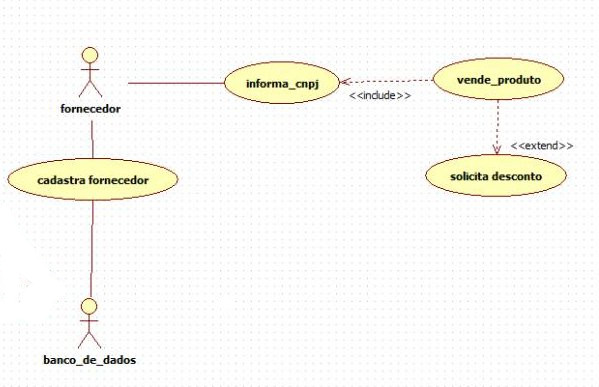
\includegraphics[scale = 0.70]{imagens/uml-fornecedor.jpg}
	\\Fonte: Do autor
\end{figure}





%=================================================================================
\newpage
\section{Fluxograma}

O fluxograma é uma representação gráfica de um processo ou rotina de trabalho geralmente feito através de figuras geométricas e retas que demonstram, de forma descomplicada, a transição de informações entre os elementos que o compõem.

Pode ser definido também como o gráfico em que se representa o curso ou caminho percorrido por certo elemento;

O fluxograma é fundamental para simplificação e racionalização do trabalho, permitindo um estudo detalhado dos métodos, processos e rotinas de um departamento ou área da organização. 


\begin{figure}[H]
	\centering 
	\caption{Floxograma}
	
	\label{loxograma}
	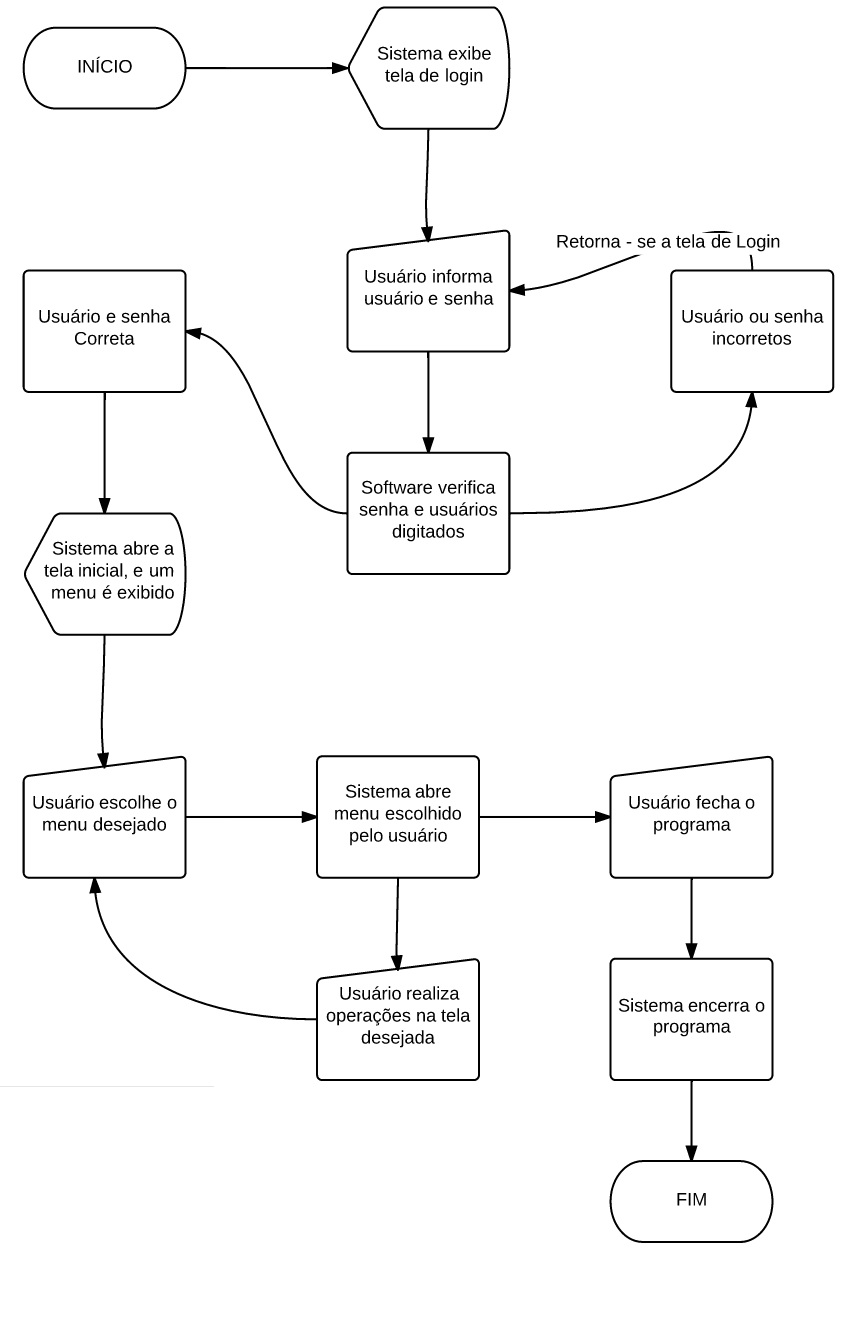
\includegraphics[scale = 0.70]{imagens/fluxo.jpg}
	\\Fonte: Do autor
\end{figure}


%===================================================================================================
\newpage
\section{Construção do Banco de dados}


\begin{figure}[H]
	\centering 
	\caption{Banco de dados Cliente}
	\label{banco_de_dados}
	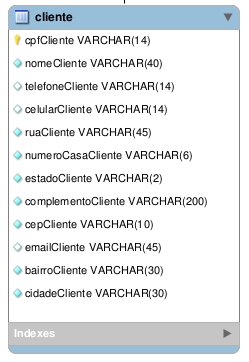
\includegraphics[scale = 0.8]{imagens/bd-cliente.png}
	\\Fonte: Do autor
\end{figure}

\begin{table}[H]
\caption{Tabela Cliente}
\begin{center}
\begin{tabular}{|c|c|c|c|c|c|}
\hline
Nome & Descrição & Tipo & Tamanho & Restrições \\ \hline
CPF & Chave primária. CPF do cliente & Char & 14 & Validar \\ \hline
Nome & Nome dos cliente & Char & 40 & - \\ \hline
Estado & Estado onde o cliente reside & Char & 2 & - \\ \hline
Cidade & Cidade do cliente reside& Char & 30 & - \\ \hline
Bairro & Bairro do cliente reside& Char & 30 & - \\ \hline
Rua & Rua da residência do cliente& Char & 45 & - \\ \hline
Número & Número da residência do cliente & Int & 6 & - \\ \hline
Celular & Celular do cliente & Char & 14 & - \\ \hline
Telefone & Telefone fixo do cliente & Char & 14 & - \\ \hline
CEP & CEP do cliente & Char & 10 & - \\ \hline
Complemento & Complemento da residência& Char & 200 & - \\ \hline
E-mail & E-mail do cliente & Char & 45 & - \\ \hline
\end{tabular}
\end{center}
\label{tabela_cliente}
\end{table}

%========================================================================================

\begin{figure}[H]
	\centering 
	\caption{Banco de dados Funcionario}
	\label{banco_de_dados}
	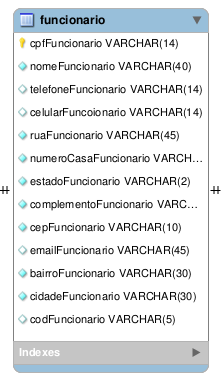
\includegraphics[scale = 0.8]{imagens/bd-func.png}
	\\Fonte: Do autor
\end{figure}


\begin{table}[H]
\caption{Tabela Funcionario}
\begin{center}
\begin{tabular}{|c|c|c|c|c|c|}
\hline
Nome & Descrição & Tipo & Tamanho & Restrições \\ \hline
CPF & Chave primária. CPF do funcionário & Char & 14 & Validar \\ \hline
Nome & Nome do funcionário & Char & 40 & - \\ \hline
Estado & Estado onde o funcionário reside & Char & 2 & - \\ \hline
Cidade & Armazena a cidade onde o funcionário reside & Char & 30 & - \\ \hline
Bairro & Bairro onde o funcionário reside & Char & 30 & - \\ \hline
Rua & Armazena a rua da residência do funcionário & Char & 45 & - \\ \hline
Número & Número da residência do funcionário & Int & 6 & - \\ \hline
Celular & Celular do funcionário & Char & 14 & - \\ \hline
Telefone & Telefone fixo do funcionário & Char & 14 & - \\ \hline
CEP & CEP do funcionário & Char & 10 & - \\ \hline
Complemento & Complemento do endereço & Char & 200 & - \\ \hline
E-mail & E-mail do funcionário & Char & 45 & - \\ \hline
\end{tabular}
\end{center}
\label{tabela_funcionario}
\end{table}



%========================================================================================

\begin{figure}[H]
	\centering 
	\caption{Banco de dados Fornecedor}
	\label{banco_de_dados}
	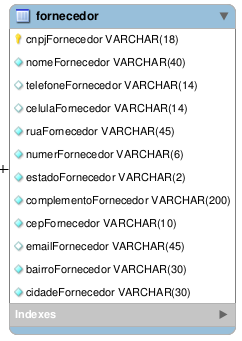
\includegraphics[scale = 0.8]{imagens/bd-fornecedor.png}
	\\Fonte: Do autor
\end{figure}

\begin{table}[H]
\caption{Tabela Fornecedor}
\begin{center}
\begin{tabular}{|c|c|c|c|c|c|}
\hline
Nome & Descrição & Tipo & Tamanho & Restrições \\ \hline
CNPJ & Chave primária. CNPJ dos fornecedores & Char & 18 & Validar \\ \hline
Nome & Nomes dos fornecedores & Char & 40 & - \\ \hline
Estado & Estado onde o fornecedor tem sede & Char & 2 & - \\ \hline
Cidade & Cidade onde é a sede dos fornecedores & Char & 30 & - \\ \hline
Bairro & Bairro onde fica a sede dos fornecedores & Char & 30 & - \\ \hline
Rua & Rua onde fica a sede dos fornecedores & Char & 45 & - \\ \hline
Número & Número da sede dos fornecedores & Int & 6 & - \\ \hline
Celular & Celular dos fornecedores & Char & 14 & - \\ \hline
Telefone & Telefone fixo dos fornecedores & Char & 14 & - \\ \hline
CEP & CEP dos fornecedores & Char & 10 & - \\ \hline
Complemento & Complemento do endereço & Char & 200 & - \\ \hline
E-mail & E-mail dos fornecedores & Char & 45 & - \\ \hline
\end{tabular}
\end{center}
\label{tabela_fornecedor}
\end{table}



%========================================================================================
\begin{figure}[H]
	\centering 
	\caption{Banco de dados Venda}
	\label{banco_de_dados}
	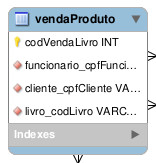
\includegraphics[scale = 0.8]{imagens/bd-venda.jpg}
	\\Fonte: Do autor
\end{figure}

\begin{table}[H]
\caption{Tabela venda de produto}
\begin{center}
\begin{tabular}{|c|c|c|c|c|c|}
\hline
Nome      & Descrição & Tipo & Tamanho & Formato \\ \hline
Código    & Chave primária. Armazena o código da venda & Int & - & Auto \\ 
Venda     &                                            &     & - & Incremento \\ \hline
CPF & Chave estrangeira de Funcionário.      & Char & 11 & - \\ 
Funcionário & Indica que funcionário efetuou a venda &       &    & \\ \hline
CPF  & Chave estrangeira de Cliente.        & Char & 11 & - \\ 
Cliente & Indica qual cliente efetuou a compra &       &    &  \\ \hline
Código  & Chave estrangeira de Livro.    & Char & 8 & - \\ 
Livro & Indica qual livro foi vendido. &       &   & \\ \hline
\end{tabular}
\end{center}
\label{tabela_venda_produto}
\end{table}


%========================================================================================

\begin{figure}[H]
	\centering 
	\caption{Banco de dados Compra}
	\label{banco_de_dados}
	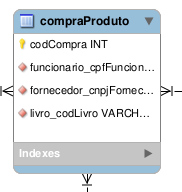
\includegraphics[scale = 0.8]{imagens/bd-compra.png}
	\\Fonte: Do autor
\end{figure}

\begin{table}[H]
\caption{Tabela compra de produto}
\begin{center}
\begin{tabular}{|c|c|c|c|c|c|}
\hline
Nome & Descrição & Tipo & Tamanho & Formato \\ \hline
Código & Chave primária de Compra de Produto. & Int & - & Auto \\ 
Compra & Armazena o código de compra.         &         &   & Incremento\\ \hline
CPF  & Chave estrangeira da entidade Funcionário. & Char & 11 & - \\ 
Funcionário & Indica qual funcionário efetuou a venda.   &       &    &  \\ \hline
CNPJ & Chave estrangeira da entidade Fornecedor.    & Char & 18 & - \\ 
Fornecedor & Indica qual fornecedor vendeu dado produto. &       &    & \\ \hline
Código & Chave estrangeira da entidade Livro.& Char & 8 & - \\ 
Livro  & Indica qual livro foi comprado.     &       &   &   \\ \hline
\end{tabular}
\end{center}
\label{tabela_compra_produto}
\end{table}


%========================================================================================--
\begin{figure}[H]
	\centering 
	\caption{Banco de dados Livros}
	\label{banco_de_dados}
	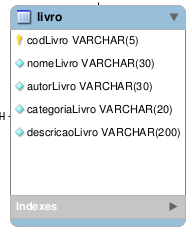
\includegraphics[scale = 0.8]{imagens/bd-livro.png}
	\\Fonte: Do autor
\end{figure}

\begin{table}[H]
\caption{Tabela Livro}
\begin{center}
\begin{tabular}{|c|c|c|c|c|c|}
\hline
Nome & Descrição & Tipo & Tamanho & Restrições \\ \hline
 Código & Chave primária. Armazena o código do livro & Char & 8 & - \\ \hline
 Nome  & Armazena o nome dos livros & Char & 30 &- \\ \hline
 Autor & Armazena o autor dos livros & Char & 30 &- \\ \hline
 Categoria  & Armazena a categoria dos livros  & Char & 20 &- \\ \hline
 Descrição  & Armazena a descrição dos livros  & Char & 200 &- \\ \hline
\end{tabular}
\end{center}
\label{tabela_livro}
\end{table}




%===================================================================================================
\newpage
\section{Detalhamento das telas do software}

\subsection{Tela login}

 A tela de login é a primeira tela a ser exibida ao usuário, foi desenvolvido com o intuito de assegurar a empresa de que somente pessoas autorizadas terão acesso as demais telas;

 \begin{figure}[H]
	\centering 
	\caption{Tela de login do software}
	\label{login software}
	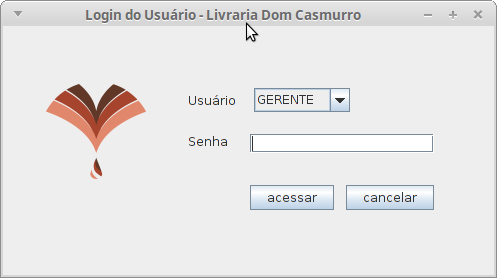
\includegraphics[scale = 0.7]{imagens/tela-login.png}
	\\Fonte: Do autor
\end{figure}

Ao abrir o software a tela de login é exibida, mostrando os campos “usuário” e “senha”;
 
\begin {itemize} 

\item No campo “usuário” terá três opções: “Gerente”, “Vendedor”, “Caixa”, e no campo “senha” terá que ser digitado: “empresa123”, essa senha é utilizada por todos os três tipos de usuários;

\itemHavendo também  dois botões, um para “cancelar” e outro “acessar” o software;

\item Se o botão “Cancelar” for pressionado é exibida uma mensagem: “Tem certeza que deseja cancelar a operação? ” se “sim” a mensagem de aviso é fechada e o programa é automaticamente encerrado;

\item Se no botão “cancelar” for pressionado juntamente com o botão “não” é fechado a mensagem de aviso, e retorna para a tela de login;

\item Se o botão “Acessar” for pressionado o software verifica se a senha está correta, a tela de login é encerrada e a tela principal do software é exibida. 

\item Caso a senha esteja incorreta, ou não foi preenchido o software exibe uma mensagem “Senha incorreta” e limpa o campo para que o usuário possa digitar novamente.
\end{itemize}


\begin{figure}[H]
	\centering 
	\caption{Tela de login do software - com mensagem}
	\label{login software}
	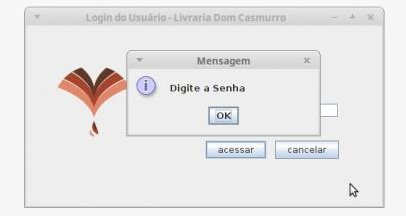
\includegraphics[scale = 0.8]{imagens/tela-login-senha.jpg}
	\\Fonte: Do autor
\end{figure}

<<<<<<< HEAD

%===================================================================================================
\subsection{Tela Principal do Software}

 Essa é a tela principal do software, todas as telas sendo de “Cadastro”, “Consulta”, “Editar”, “Deletar” ou “Sobre” 
 são inseridos sobre a tela principal, nela são exibidos os menus e os submenus das operações como “Cliente”, “Funcionário”,
 “Fornecedor”, “Livros”. Optamos por deixar  simples seu manuseio. Fazendo com que qualquer pessoa leiga na área da informática
 possa realizar as operações sem dificuldades;
 
 \begin{figure}[H]
	\centering 
	\caption{Tela principal do software}
	\label{tela-principal}
	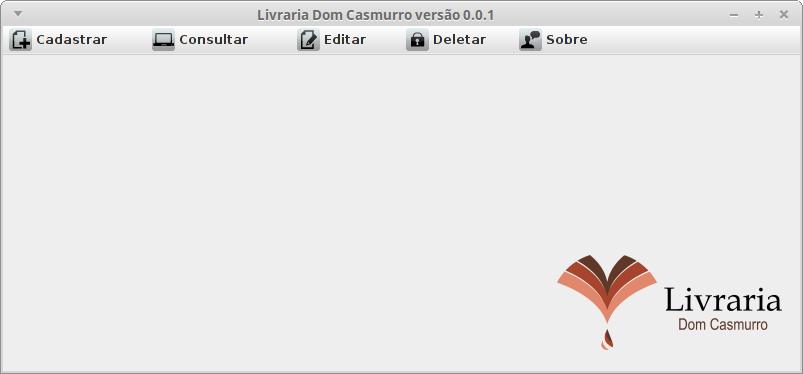
\includegraphics[scale = 0.6]{imagens/tela-principal.png}
	\\Fonte: Do autor
\end{figure}
 
 
 \begin{itemize}
  \item Na tela principal do software exibe um menu com as seguintes informações “Cadastrar”, “Consultar”, “Editar”,
  “Deletar”, “Sobre”;
  
  \item Entre as opções  “Cadastrar”, “Consultar”, “Editar”, “Deletar”,  ao ser selecionada será exibido um submenu com as 
  informações respectivamente:   “Cliente”, “Funcionário”, “Fornecedor”, “Livros”, onde poderá executar as demais operações;
 \end{itemize}
 
 
 \begin{figure}[H]
	\centering 
	\caption{Tela principal do software com os submenus}
	\label{principal-menu}
	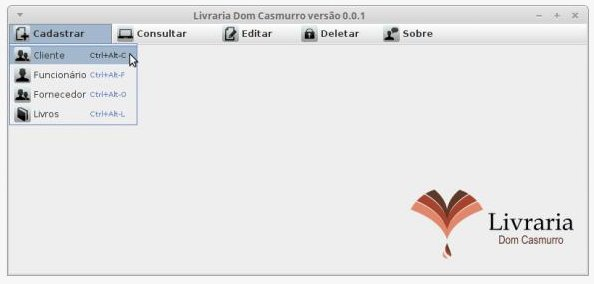
\includegraphics[scale = 0.8]{imagens/tela-principal-menu.jpg}
	\\Fonte: Do autor
\end{figure}



%===================================================================================================
\subsection{Tela de Cadastro}

Os Clientes, funcionários, fornecedores, e os livros terão respectivamente sua tela de cadastro, nela o funcionário 
da empresa preenchera com os dados em cada uma das TextField apresentadas em suas telas, após preencher os dados, o 
programa seleciona os campos e armazena as informações digitadas na base de dados;

\begin{itemize}
 \item Se o usuário pressionar a opção do menu “cadastrar”, exibe os submenus de “Cliente”, “Funcionário”, “Fornecedor”, “Livros”;
 \item Em todas as telas de “Cadastro” conterá dois botões um “Cadastrar” e “Cancelar”;
\end{itemize}

 \begin{figure}[H]
	\centering 
	\caption{Tela de cadastro - Exemplo Cliente}
	\label{cadastro_cliente}
	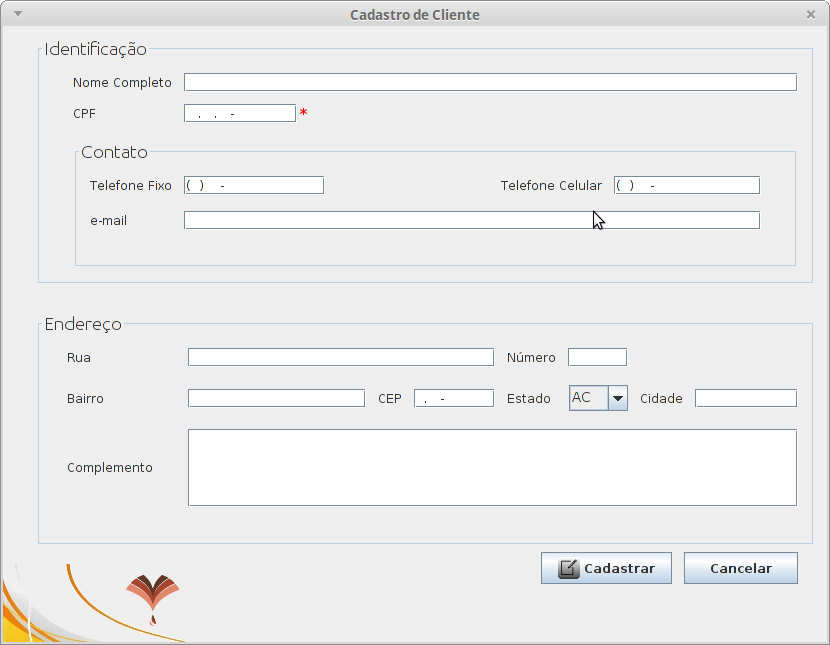
\includegraphics[scale = 0.5]{imagens/cadastro-cliente.png}
	\\Fonte: Do autor
\end{figure}

\begin{figure}[H]
	\centering 
	\caption{Tela de cadastro - Exemplo Livro}
	\label{cadastro_livro}
	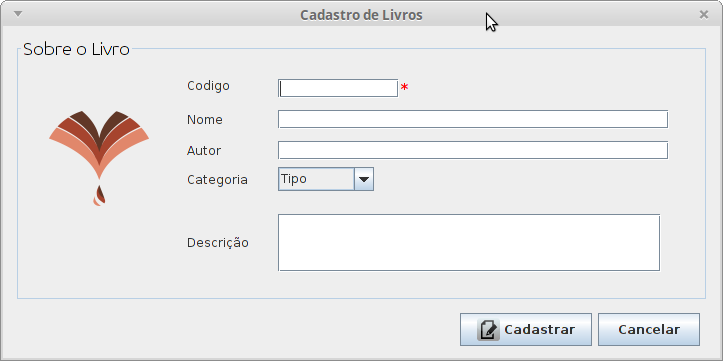
\includegraphics[scale = 0.6]{imagens/cadastrar-livro.png}
	\\Fonte: Do autor
\end{figure}


\begin{itemize}
 \item Se o botão selecionado for “Cadastrar”, o programa verifica se o  CPF e o nome foram preenchidos, se “não” é exibido uma mensagem de aviso: “Insira o nome ou CPF”; se “sim” retem as informações e armazenas no banco de dados;

 \item Outra precalçam feita no software é na verificação se o CPF já foi armazenado no banco de dados, se “sim” retorna uma mensagem de aviso : “Cliente já cadastrado”;

  \item Se o botão pressionado for “Cancelar”  é exibida uma mensagem: “Tem certeza que deseja cancelar a operação? ” se “sim” a mensagem de aviso é fechada e o programa retorna para a tela principal; Se “não” a mensagem é fechada e permanece na tela de cadastro;

\end{itemize}




%===================================================================================================
\subsection{Tela de Consulta}

A  tela de consulta foi criada para auxiliar a empresa nas consultas de seus cadastros, cada classe possui
um atributo principal sendo eles: 


\begin{table}[H]
\centering
\begin{tabular}{|c|c|}\hline
\textbf{Classe} & \textbf{Atributo Principal}\\\hline
Cliente & CPF\\\hline
Funcionário & CPF\\\hline
Fornecedor & CNPJ\\\hline
Livros & CODIGO DO LIVRO\\\hline
\end{tabular}
\end{table}

Esse atributos terão que ser digitados para que a consulta seja executada, pois seleciona o atributo principal
e verifica se foi cadastrado no banco de dados;

\begin{itemize}
 \item Se o usuário pressionar a opção do menu “consultar, exibe os submenus de “Cliente”, “Funcionário”, “Fornecedor”, “Livros”;


 \item Em todas as tela de “Consulta” será exibido um campo para que o usuário preencha com o atributo principal de cada uma das operações;

 \item Os demais campo como os de “Nome”,  “Telefone fixo”, “Telefone Celular”, “e-mail”, “Rua”, “Número”, “Bairro”, “Estado”, “Cidade”, “CEP”, “Complemento” ficam inativos, o usuário não consegue digitar nada nesses campos somente no atributo principal;
\end{itemize}

\begin{figure}[H]
	\centering 
	\caption{Tela de consulta - Exemplo Cliente}
	\label{consulta_cliente}
	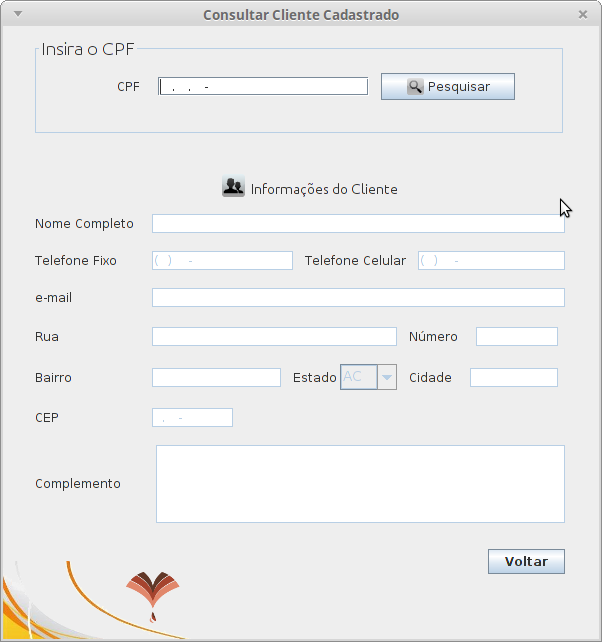
\includegraphics[scale = 0.6]{imagens/tela-consulta-cliente.png}
	\\Fonte: Do autor
\end{figure}


\begin{figure}[H]
	\centering 
	\caption{Tela de consulta - Exemplo Livro}
	\label{consulta_livro}
	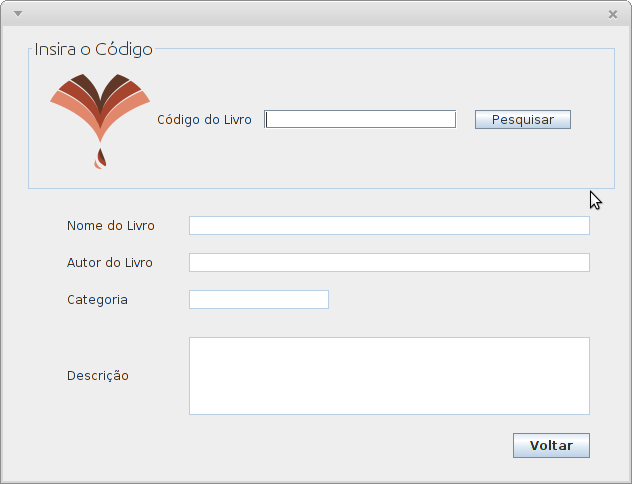
\includegraphics[scale = 0.6]{imagens/tela-consulta-livro.png}
	\\Fonte: Do autor
\end{figure}



\begin{itemize}
 \item Após digitar o atributo principal o usuário pressiona o botão pesquisar. Pois os outros botões e os campos ficam inativos, onde impede que o usuário pressione ou digite algo neles;

 \item Ao ser pressionado o pesquisar o programa verifica no banco de dados se existe algum cliente com aquele determinado CPF, se “sim” retorna os dados do cliente. Se na busca o programa não encontrar nenhum cadastro feito com o CPF digitado, é exibido uma mensagem: “Cliente não cadastrado”; 

 \item Se nesta mesma tela o for pressionado o botão “voltar”, a tela atual de consulta é fechada e volta para a tela principal;
\end{itemize}


%===================================================================================================
\subsection{Tela de Editar}

A  tela de editar foi criada com o intuito de auxiliar os funcionários da empresa a fazer edições dos cadastros, por exemplo:
um cliente mudou de endereço, o funcionário faz a pesquisa no banco de dados, e tem acesso as informações deste cliente, e pode
editar as informações como o do endereço;

\begin{itemize}
 \item Se for pressionar a opção do menu “editar”, também são exibidos os submenus de “Cliente”, “Funcionário”, “Fornecedor”, “Livros”; 
\end{itemize}

\begin{figure}[H]
	\centering 
	\caption{Tela de editar - Exemplo Cliente}
	\label{editar_cliente}
	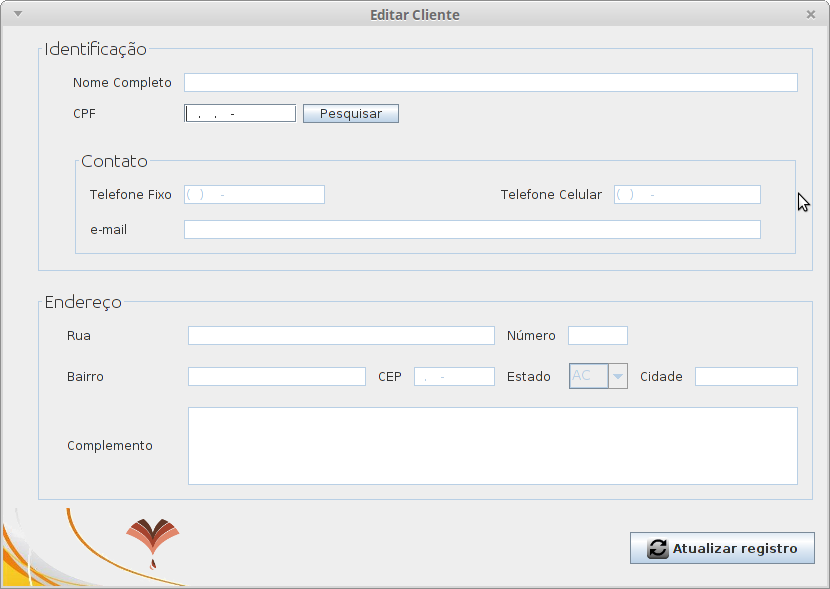
\includegraphics[scale = 0.6]{imagens/tela-editar-cliente.png}
	\\Fonte: Do autor
\end{figure}

\begin{itemize}
 \item Todos os campos ficam inativos, enquanto o usuário não digitar o atributo principal, e ele for encontrado na base de dados;

 \item Se o atributo principal for cadastrado no software ao pesquisar ele retorna os dados do cliente, e os campo deixam de ser inativos e retorna os dados do cliente, caso seja necessário a edição de algum campo o usuário deleta o que foi digitado ou acrescenta e atualiza no banco de dados com o botão;

 \item O botão “atualizar registro”, é utilizado para atualizar no banco de dados a nova informação do cliente. Com o seguinte código:
 \end{itemize}
 
 
 %===================================================================================================
\subsection{Tela de Deletar}

Tela criada para auxiliar o funcionário remover os registros cadastrados no banco de dados;

\begin{itemize}
 \item Se for pressionada a opção do menu “deletar”, também são exibidos os submenus de “Cliente”, “Funcionário”, “Fornecedor”, “Livros”;

  \item Todos os campos ficam inativos, enquanto o usuário não digitar o atributo principal, e ele for encontrado na base de dados;
  
  \item Logo após isso os dados são retornados caso encontrados, e o usuário poderá remover o cadastro clicando no botão deletar
 \end{itemize}

\begin{figure}[H]
	\centering 
	\caption{Tela de deletar - Exemplo Cliente}
	\label{Deletar_cliente}
	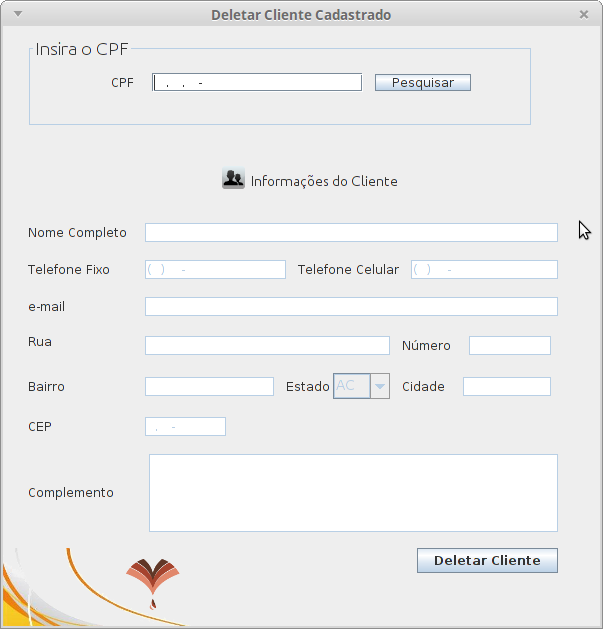
\includegraphics[scale = 0.6]{imagens/tela-deletar-cliente.png}
	\\Fonte: Do autor
\end{figure}


 %===================================================================================================
\subsection{Tela do Sobre}

Mostra as informações do desenvolvedor do software;

\begin{figure}[H]
	\centering 
	\caption{Tela do sobre}
	\label{sobre}
	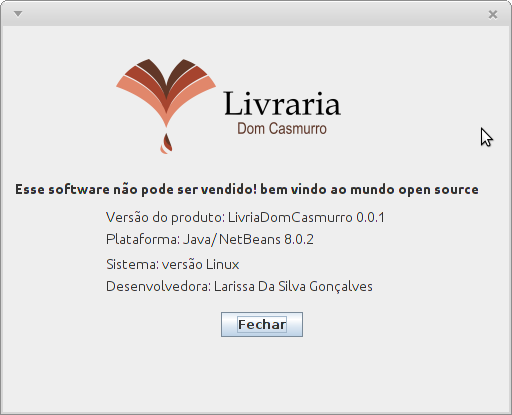
\includegraphics[scale = 0.6]{imagens/tela-sobre.png}
	\\Fonte: Do autor
\end{figure}

